\chapter{Metodologia}
\label{chap:metodologia}

O Gráfico 1 apresenta a distribuição anual da produção, realizando-se uma comparação entre a produção de dissertações de mestrado e teses de doutorado.

    \begin{figure}[h!]
    	\centering
    	\Caption{\label{fig_mapa-3} Produção anual das dissertações de mestrado e teses de doutorado entre os anos de 1990 e 2008}    	
    	\IBGEtab{}{
    		\fbox{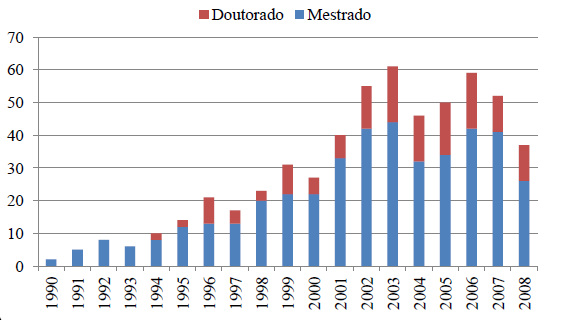
\includegraphics{figuras/figura-3}}
    	}{
    		\Fonte{os autores}
    		\Nota{Esta é uma nota, que diz que os dados são baseados na
    		regressão linear}
    		\Nota[Anotações]{Uma anotação adicional, seguida de várias outras.}
    	}
    \end{figure}

Nota-se a partir do Gráfico 1 e da Tabela 1 que a produção de teses de doutorado teve seu início no ano de 1994, esta informação se justifica devido ao fato de que os cursos de doutorado na \index{área} da Saúde Coletiva começaram a surgir no país a partir do ano de 1990, que coincide com o ano de implantação do SUS. As duas primeiras teses com o ano de 1994 fazem parte do doutorado em Saúde Coletiva da UNICAMP e do Doutorado em saúde Pública da USP. Nos \index{anos} de 2003 e 2006, houve uma produção mais elevada no que diz respeito às \index{teses} de doutorado, se comparada com a produção dos outros anos. Observa-se também que 2003 e 2006 são os anos de maior pico de produção científica de temas relacionados ao campo do trabalho.

As instituições que possuem cursos de doutorado que tiveram teses publicadas na área do trabalho são: Doutorado em Saúde Coletiva do Instituto de Medicina Social da UERJ; doutorado em Saúde Pública da Escola Nacional de Saúde Pública da FIOCRUZ; Doutorado em Saúde Coletiva da UNICAMP; \index{Doutorado} em Saúde Coletiva e Saúde Pública da UFBA; Doutorado em Saúde Pública e Epidemiologia da USP; Doutorado em Saúde Pública da UFMG; Doutorado em Epidemiologia da UFPEL [...]

Foi possível identificar a \index{distribuição} das dissertações e teses ao longo do período pesquisado. A Tabela 1 apresenta a produção de mestrado e doutorado em cada ano analisado.

 	\begin{table}[h!]
    	\centering
    	\Caption{\label{fig_mapa}Produção anual das dissertações de mestrado e teses de doutorado entre os anos de 1990 e 2008}    	
    	\IBGEtab{}{
    		\begin{tabular}{cll}
   				\toprule
   				Ranking & Exon Coverage & Splice Site Support\\
   				\midrule \midrule
  				E1 & Complete coverage by a single transcript & Both splice sites\\
  				E2 & Complete coverage by more than a single transcript & Both splice sites\\
   				E3 & Partial coverage & Both splice sites\\
   				E4 & Partial coverage & One splice site\\
   				E5 & Complete or partial coverage & No splice sites\\
   				E6 & No coverage & No splice sites \\
   				\bottomrule
   			\end{tabular}
    	}{
    		\Fonte{os autores}
    		
    	}
    \end{table}
    
Foi possível identificar a distribuição das dissertações e teses ao longo do período pesquisado. A Tabela 1 apresenta a \index{produção} de mestrado e doutorado em cada ano analisado.

\begin{quadro}[h!]
	\centering
	\Caption{\label{quadro:exemplo-de-um-quadro}Produção anual das dissertações de mestrado e teses de doutorado entre os anos de 1990 e 2008}	
	\IBGEtab{}{
		\normalsize
		\begin{tabular}{|c|c|c|}
			\hline
			Nome/Sobrenome & Descrição do texto & Conclusão \\ \hline
			Manoel & Modelo de Quadro & Quadro confeccionado \\ \hline
			Alves & Modelo de Quadro & Quadro confeccionado \\ \hline 
			Damascena & Modelo de Quadro & Quadro confeccionado \\ \hline
			Júnior & Modelo de Quadro & Quadro confeccionado \\ \hline
		\end{tabular}
	}{
	\Fonte{os autores}
}
\end{quadro}

\lipsum[3]

\section{Exemplo de citação longa}

Segundo definição da Universidade Federal de São Paulo-UNIFESP (2013, p. 6),

\begin{citacao}
Trabalho acadêmico é o documento exigido como aproveitamento de uma disciplina, curso ou programa, baseado no estudo de um assunto por meio de pesquisa cientifica, como resultado de alguns dos diversos processos ligados à produção e transmissão de conhecimento executados no âmbito das instituições [de] ensino, pesquisa e extensão, formalmente reconhecidas para o exercício dessas atividades.
\end{citacao}

No concernente ao tema, apresenta-se a NBR 14724 da ABNT (2011) que versa sobre informação e documentação de trabalhos acadêmicos visando a apresentação destes à instituição (banca, comissão examinadora e outros).

\section{Exemplo de notas de rodapé}

Deve-se utilizar o sistema autor-data para as citações no texto \footnote{Veja-se como exemplo desse tipo de abordagem o estudo de Netzer (1976).} e o numérico para notas explicativas. As notas de rodapé podem e devem ser alinhadas, a partir da segunda linha da mesma nota, abaixo da primeira letra da primeira palavra, de forma a destacar \footnote{Encontramos esse tipo de perspectiva na 2ª parte do verbete referido na nota anterior, em grande parte do estudo de Rahner (1962).} o expoente e sem espaço entre elas e com fonte menor (tamanho 10).


\section{Exemplo de Funções Matemáticas}

One of the greatest motivating forces for Donald Knuth when he began developing the original TeX system was to create something that allowed simple construction of mathematical formulas, while looking professional when printed. \autoref{equacao-1}

\begin{equation}
	\label{equacao-1}
	\begin{aligned}
		& \text{Minimizar (ou Maximizar)}
		& & f(x) \\
		& \text{sujeito a}
		& & g_i(x) \leq 0 \text{ para } i=\{1,2,3,...,m\} \\
		&&& h_j(x) = 0 \text{ para } j=\{1,2,3,...,p\} \\
		&&& x \in \Omega
	\end{aligned}
\end{equation}

ou ainda a \autoref{equacao} The fact that he succeeded was most probably why TeX (and later on, LaTeX) became so popular within the scientific community. Typesetting mathematics is one of LaTeX's greatest strengths. It is also a large topic due to the existence of so much mathematical notation.

\begin{equation}
	\label{equacao}
	\lim_{x \to \infty} \exp(-x) = 0
\end{equation}

Became so popular within the scientific community. Typesetting mathematics is one of LaTeX's greatest strengths. It is also a large topic due to the existence of so much mathematical notation.